
\resetcounters
\bibliographystyle{asp2010}

\markboth{Landais, Ochsenbein, and Simon}{TAPVizieR: A New Way to Access the VizieR Database}

\resetcounters

\title{TAPVizieR: A New Way to Access the VizieR Database}
\author{Gilles~Landais, Fran\c cois~Ochsenbein, Anne-Camille~Simon
\affil{Centre de Donn\'ees astronomiques de Strasbourg (CDS) }}

\aindex{Landais, G.}
\aindex{Ochsenbein, F.}
\aindex{Simon, A.-C.}

\begin{abstract}
VizieR is a component of the Virtual Observatory: it provides tables of
catalogs to external software with VO standards like the VOTable output.
Accessing VizieR with the ADQL/TAP standard represents a new milestone
in the VizieR access facilities.

The PostgreSQL engine has been chosen to store data: it provides a solid
database containing utilities to manage SQL or to create the customized
HEALPix\ooindex{HEALPix, ascl:1107.018} indexing ``H3C'' which permits fast access from sky coordinates.
The TAP standard however was not designed to accommodate databases
managing tens of thousands of tables like VizieR, and some compromises
with the TAP standard were necessary in this first version of TAPVizieR.
\end{abstract}

\section{The context}

ADQL \citep{adql_2011} is an other way to query VizieR tables 
\citep{ochsenbein_2000}; ADQL is an extension of SQL 
with additional astronomical functions and geometrical objects. 
It enables the usage of formulae involving column combinations which can be used 
for display or to filter a set of records (see Figure~\ref{P044:ADQLexample}). 
These kinds of operations were limited in the VizieR application and required 
the usage of external software for such computations.

\begin{figure}[!h] \center
\begin{footnotesize}
\begin{verbatim}
SELECT ra_icrs_, de_icrs_, BTmag-VTmag as B-V
FROM   tyc2
WHERE  1=CONTAINS(POINT('ICRS', ra_icrs_, de_icrs_),
                  CIRCLE('ICRS', 244.26, -22.98, 10/60.))
   AND BTmag-VTmag<1
\end{verbatim}\end{footnotesize}
\caption{Example of an ADQL query on the catalog Tycho using a color 
constraint (BTmag-VTmag) and a cone search arround M80.}\label{P044:ADQLexample}
\end{figure}

TAP \citep{tap_2011} is a protocol to execute an ADQL query 
on a remote database. 
TAP services are already available in data centers like CADC or GAVO, and
some external software like TOPCat\ooindex{TOPCAT, ascl:1101.010} or TAPHandle can work with
the standard. These applications link tables coming from different databases
(GAVO, CADC and now VizieR) with a unique interface and use the same language.
They offer real extended possibilities for astronomers who can combine 
tables stored in different places. %data center.


\section{A Dedicated Database}

\subsection{Homogenize the Storage}
The VizieR application provides catalogs. The tables and their metadata (descriptions) 
are stored in a transactionnal database, or in dedicated binary files
for the large catalogs (e.g. WISE, 2MASS, SDSS, etc.) in order to speed up the 
search by position.

ADQL based on SQL requires a
transactional database or 
technologies like Hadoop. We think that SQL is the more practical way
to be ADQL-compatible, so, we chose to create a new dedicated database which
gathers all catalogs. 

This new database is a PostgreSQL engine which effectively supports 3.5 Tb
of data and indexes.
With PostgreSQL, we gain the replication capabilities and some easy way
to create advanced functions.

\subsection{Indexation}
VizieR has tables that can contain up to 1 billion records. This volumetry
needs indexation and in particular a positional indexation, because conesearch
or crossmatch (join tables according to their positions) are the most popular 
functionalities in VizieR.

In PostgreSQL an index by position can be built with libraries like PgSphere
provided by PostgreSQL; an external plugin Q3C
was also developed 
by \citet{q3c_2006} for astronomical applications.
The PgSphere is user-friendly; however, Q3C minimizes resources and
is more efficient with tables containing over one million records ---
therefore better suited for VizieR.
Q3C works with the quadcube algorithm;
however, {\em HEALPix}\ooindex{HEALPix, ascl:1107.018} is more and more becoming a standard in
astronomical applications like 
Aladin\ooindex{Aladin, ascl:1112.019}, the CDS Crossmatch service, GAIA, etc.


\paragraph{The H3C library}

We built a 2D PostgreSQL library \textbf{H3C} 
(\textit{i.e. \textbf{H}ealpiX-\textbf{T}ree-C code}), largely inspired from
 Q3C, with the same functionalities --- with the exception that
the functions dealing with polygons are available 
for convexes only.

The tessellation of the sphere with HEALPix\ooindex{HEALPix, ascl:1107.018} cells requires however
a deep resolution 
to be as efficient as Q3C. This implementation was possible thanks to the recent
improvement of the  HEALPix\ooindex{HEALPix, ascl:1107.018} 64bits C++ library maintained by NASA 
\citep{gorski_healpix}.

\paragraph{Some comparisons between libraries} (see Figure~\ref{P044:comparative})
Regarding  efficiency, the tests show that Q3C and H3C are largely better than 
PgSphere. Moreover the size required by the index
as well as the time required for their creation,
are significantly smaller with Q3C/H3C than with PgSphere.

\begin{figure}[htp] \center
\begin{small}
\begin{tabular}{lllll}
 & PgSphere & Q3C & H3C & H3C  \\
 &          &     &     &{\scriptsize cluster index} \\
conesearch in 2mass (M1, radius:2arcsec) & 340ms& 360ms& 380ms &\\
conesearch in 2mass (M1, radius:2arcmin) & 500ms& 390ms& 400ms &\\
conesearch in 2mass (M1, radius:2deg)    & 88s& 4.3s& 1.26s &\\
crossmatch Tycho-hipparcos & 110s & 4.5s &  4.5s & 3s\\ 
crossmatch 2mass-hipparcos & 48min & 15min & 14min & 6.5min\\ 
crossmatch 2mass-Tycho     & 4h30 & 49min  & 48min & 11.5min\\ 
\end{tabular}
\end{small}
\caption{Comparisons of the positional indexation applied to Hipparcos 
($\sim$100K records), Tycho ($\sim$2.5M records) and 2mass ($\sim$450M records)
catalogues. All tests are performed on the same Linux computer (99G RAM) using a
PostgreSQL (version 9.1) database. The cache disk was deleted before each test.}
\label{P044:comparative}
\end{figure}

\paragraph{Managing the coordinate systems}

The coordinate system used in VizieR tables depends on the catalog, but VizieR 
can compute positions of any catalog in another coordinate system than the 
original one, taking into account the proper motions when these are 
described in the VizieR METAdata.

Working with a unique coordinate system is obviously more efficient
in ADQL, especially for crossmatches. So, we are adding the position in 
the ICRS frame in each table; 
the new columns (\_ra.icrs, \_de.icrs) are computed for the epoch J2000 
if proper motions are known.


\section{TAPVizieR Implementation}

\subsection{Technologies and the Library Used}
\paragraph{The database}


The TAPVizieR service uses a PostgreSQL database and takes advantage of the
C-functions to index positions using H3C;  functions dealing with 
coordinate conversions were also added on the server side.

\paragraph{Parsing the ADQL query and providing data with TAP}

The TAP/ADQL service is a Web application written in Java. 
We use the UWS/TAP and ADQL libraries \citep{simbad_tap_2011}, 
which were helpful in translating ADQL into an object tree to 
easily handle the VizieR METAdata. 

\paragraph{Architecture}
The TAPVizieR architecture is composed of the TAP/ADQL web application, a VizieR
mirror and a PostgreSQL installation (see Figure~\ref{P044:architecture}).
The database is composed of a master and a standby database using
the synchronous replication available in PostgreSQL since version 9.1.
The pool {\em PgBouncer} is also used to manage database connections, and to
enable a precise configuration. 

\begin{figure}[hbp] \center
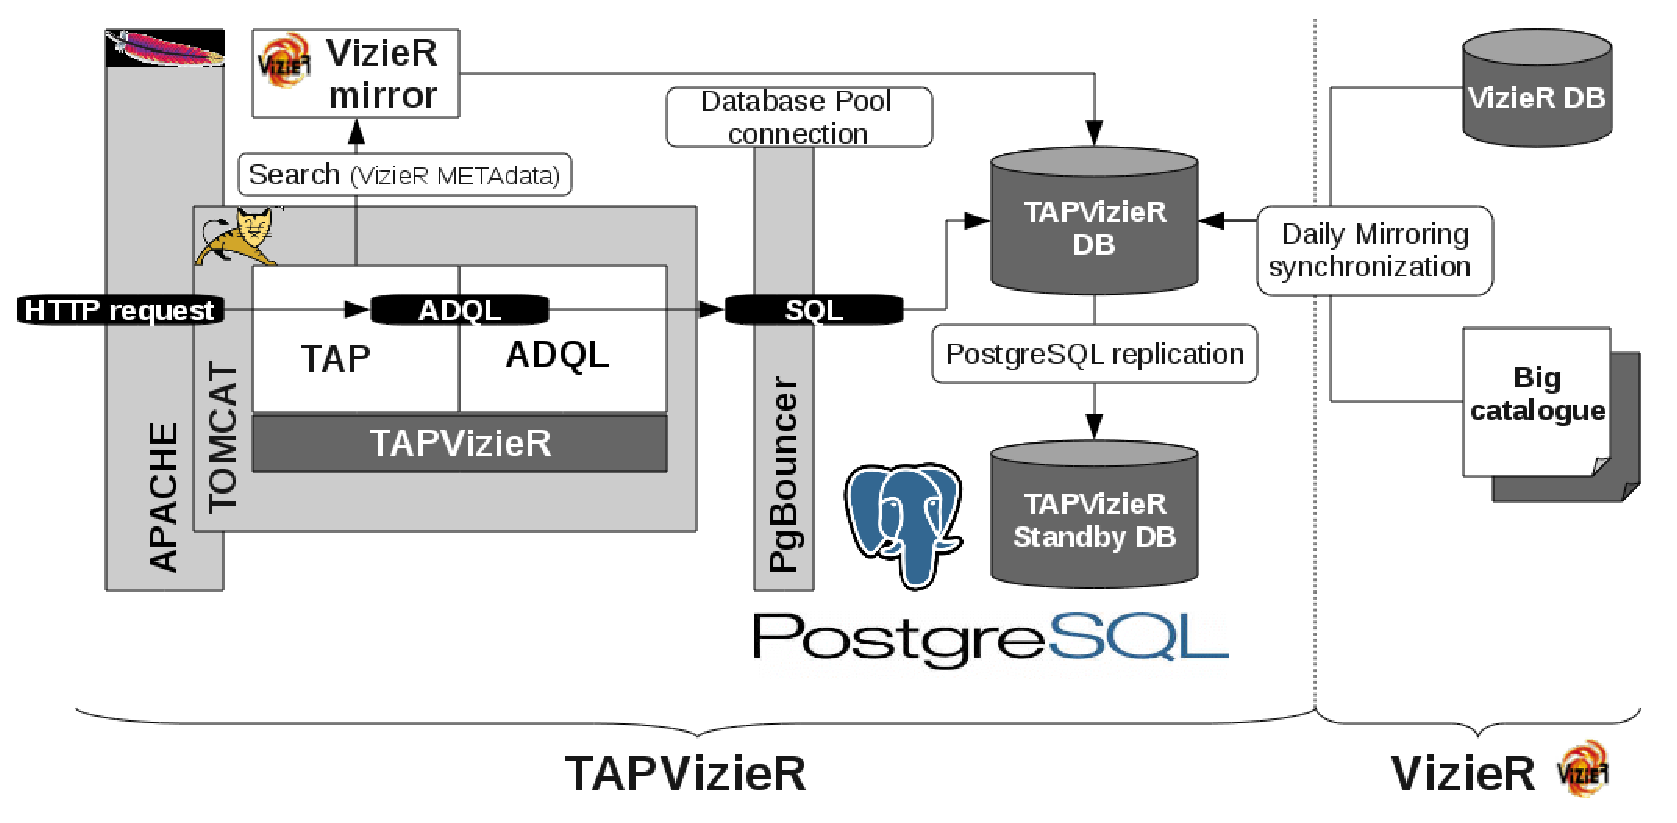
\includegraphics[width=0.85\textwidth]{part8/Landais_P44/P044_fig1.eps}
\caption{The TAPVizieR architecture}\label{P044:architecture}
\end{figure}

\subsection{The Web interface}
\label{P044:web_interface}
Two modes are available to query tables in TAPVizieR.
The first, the {\em TAP mode}, 
follows the TAP protocol; it consists of a set of standardized URLs
which
describe and execute an ADQL Query. This mode, used by external TAP-compatible
software, is available from
{\small\url{http://tapvizier.u-strasbg.fr/TAPVizieR/tap/(tap_service_name)}}

The second mode consists in a web interface  
available at {\small\url{http://tapvizier.u-strasbg.fr/adql/}}, where
commonly used ADQL queries can easily be generated.

The technologies used are Ajax/JQuery/JSON to query TAPVizieR in asynchronous 
TAP mode. The web mode uses some TAP extension, like a \textit{"/search"} service
in which the rich METAdata available in VizieR are used in order to retrieve tables 
from position, keywords, authors, etc.


\subsection{Departures from Standards}

\paragraph{A big volumetry}

The VizieR database is huge:  3.5Tb constituted by 10,000 catalogues, 20,000
tables and more than 300,000 columns of tables. The TAP standard requires
to return the TAP schema as a single XML output file. Such an output represents
$\sim$86Mb, which is too huge to be processed by remote TAP-aware
software (in 
particular for a remote web application).

So, VizieR currently returns only the table descriptions without the 
column description ($\sim$3.5Mb). 
An additional service (i.e. another URL) provides a full
description of a specified table; this service is not (yet) a TAP standard.

\paragraph{Understanding the coordinate system}

TAPVizieR makes the expected change of coordinate system in a join of 
geometrical  areas. However, the coordinate system stored in the VizieR 
METAdata is used even if the ADQL query specifies another system.

The ADQL {\em POINT} function can currently be used %in output 
to perform a change of coordinate system in the output parameters.
This syntax is not ADQL-compliant and  will evolve in the future with
the ADQL evolutions.

\section{On-going Developments}

The homogenization of tables in the same coordinate system is being performed. %have to be done.
The {\em Upload} capabilities, described in TAP, will be implemented soon.
Finally, we will add a search by {\em MOC}  (Multi-Order Coverage map) 
using the HEALPix\ooindex{HEALPix, ascl:1107.018} indexation \citep{O13_adassxxii}.

\bibliography{editor}
